% 鋭化する場所を学習する — main.tex の日本語版（確認用）
%
% 体裁は main.tex と同一（IEEE 2 段組、会議テンプレート）。本文だけを日本語にした
% もので、投稿物ではない。提出は英語版の main.tex。
%
% 日本語の組版には LuaLaTeX が要る。pdflatex では通らない:
%     ./build_ja.sh      (lualatex を 2 パス)
%
% 数値は main.tex と完全に一致させること。片方だけ直すと必ずずれる。
\documentclass[conference]{IEEEtran}
\IEEEoverridecommandlockouts

% LuaLaTeX は Times (ptm) を TU エンコーディングで見つけられず Latin Modern に
% 落ちる。英語版と字面を揃えるため、Times 互換の TeX Gyre Termes を明示する。
\usepackage{fontspec}
\setmainfont{texgyretermes}[
  Extension=.otf, UprightFont=*-regular, BoldFont=*-bold,
  ItalicFont=*-italic, BoldItalicFont=*-bolditalic]
\usepackage{luatexja}
\usepackage[haranoaji]{luatexja-preset}
\usepackage{cite}
\usepackage{amsmath,amssymb,amsfonts}
\usepackage{graphicx}
\usepackage{booktabs}

\newcommand{\bfone}{BF\textsubscript{1}}

\begin{document}

\title{拡散単眼深度推定における選択的な境界鋭化}

\author{\IEEEauthorblockN{TODO 著者名}
\IEEEauthorblockA{\textit{TODO 専攻・学科} \\
\textit{TODO 大学}\\
TODO 市, 国 \\
TODO メールアドレス}}

\maketitle

\begin{abstract}
拡散モデルに基づく単眼深度推定は面の精度は高いが、深度の不連続（物体境界）が
ぼやける。分割モデルが見つけた輪郭で予測深度を鋭化するのが自然な対処だが、
すべての輪郭に鋭化を掛けると NYUv2 の境界 \bfone{} は 1.90\% 悪化する。
本研究は測定によって、問題が輪郭の\emph{位置}ではないことを示す。真の深度段差から
最寄りの輪郭までは中央値 1.00\,px である。問題は\emph{どの輪郭を使うか}にあり、
輪郭画素の 79.8\% は 8 画素窓の中に段差を一つも持たない。正解データを使って、
真の段差から 1 画素以内にある 6.07\% だけを残し、輪郭を 1 画素も動かさずに鋭化すると、
効果は $-1.90\%$ から $+43.39\%$ へ符号が反転する。そこで本研究は修正操作を固定し、\emph{それをどこに掛けるか}だけを学習する。
NYUv2 654 枚・16 分で学習した 193 万パラメータの選別器は、\bfone{} を seed 4 本で
$11.92 \pm 0.90\%$ 向上させる。同じ 4 つの選別器を\emph{再学習なしで}、アーキテクチャも出力表現も異なる
第二の深度モデルに適用すると、そちらでは $27.83 \pm 1.27\%$ 向上する。
学習を伴わない対照 5 種を各モデル自身の予測で測定し、学習の寄与を 10.7 ポイントと
17.4 ポイントと特定した。選別器と鋭化の追加コストは深度モデルの 495\,ms に対し 1 枚あたり 30\,ms である。
分割モデルがさらに点グリッドに応じて 534〜2{,}603\,ms を加えるが、
最も粗いグリッドで利得の 91\% が得られる。
併せて負の結果も報告する。本手法は深度モデルをまたいでは転移するが、
データセットをまたいでは転移せず、試した対処はいずれも失敗した。
\end{abstract}

\begin{IEEEkeywords}
単眼深度推定, 深度境界, 後処理, 拡散モデル
\end{IEEEkeywords}

\section{はじめに}

事前学習済みの拡散モデルを転用した単眼深度推定 \cite{marigold,lotus,marigoldv2} は
画素単位の精度では強いが、生成モデルの持つ滑らかさを物体境界で引き継いでしまう。
AbsRel が優秀でありながら、画像中のすべての遮蔽境界が数画素にわたってにじんでいる、
ということが起こりうる。画素平均の指標はこれを検出しない。境界画素は画像のごく一部で、
平らな面に支配された指標は問題なしと報告するからである。
境界専用の指標なら検出できる \cite{depthpro}。

深度モデルに手を入れずに済むため、境界を後処理で直す方針は魅力的である。
先行研究は\emph{深度をどう動かすか}を学習してきた \cite{ramamonjisoa,sharpnet,edgeguided}。
本研究は逆の分解を取る。\textbf{修正操作を固定し、それをどこに掛けるかだけを学習する。}

この選択は経験的なものである。第 \ref{sec:diagnosis} 節では、分割モデル \cite{sam} が
描いた輪郭すべてに鋭化を掛けると、Marigold V2 \cite{marigoldv2} の境界 \bfone{} が
1.90\% \emph{下がる}ことを測定する。
同じ測定が理由も示す。輪郭の位置はすでに十分であり、一方で輪郭の 79.8\% は深度段差を
まったく示していない。そこを鋭化しても滑らかな面を壊すだけである。位置を一切変えずに、
正解データで正しい輪郭だけを選ぶと、効果は $-1.90\%$ から $+43.39\%$ へ動く。
ボトルネックは位置精度ではなく\textbf{選別}である。

本研究の貢献は次の 4 点である。

\begin{enumerate}
\item 後処理による境界鋭化のボトルネックが選別であることを測定で特定した。輪郭を 1 画素も
      動かさずに効果の符号を反転させるオラクルを含む（第 \ref{sec:diagnosis} 節）。
\item 修正操作を固定して選別だけを学習する手法を提案した。これにより\textbf{学習が何に
      寄与したかの帰属が明確}になる（第 \ref{sec:method} 節）。
\item アーキテクチャ・パラメータ数・出力表現の異なる 2 つの深度モデルで評価した。
      各 seed 4 本、学習を伴わない対照 5 種を\textbf{各モデル自身の予測で}
      測定した（第 \ref{sec:experiments} 節）。
\item 計算コストを分析し、追加分が 1 枚 30\,ms であること、粗い分割グリッドで
      分割コストの 20\% から利得の 91\% が得られることを示した（第 \ref{sec:cost} 節）。
\end{enumerate}

第 \ref{sec:limitations} 節では、本手法がデータセットをまたいでは転移しないこと、
およびその修復を試みて失敗したことを報告する。

\begin{figure*}[t]
\centerline{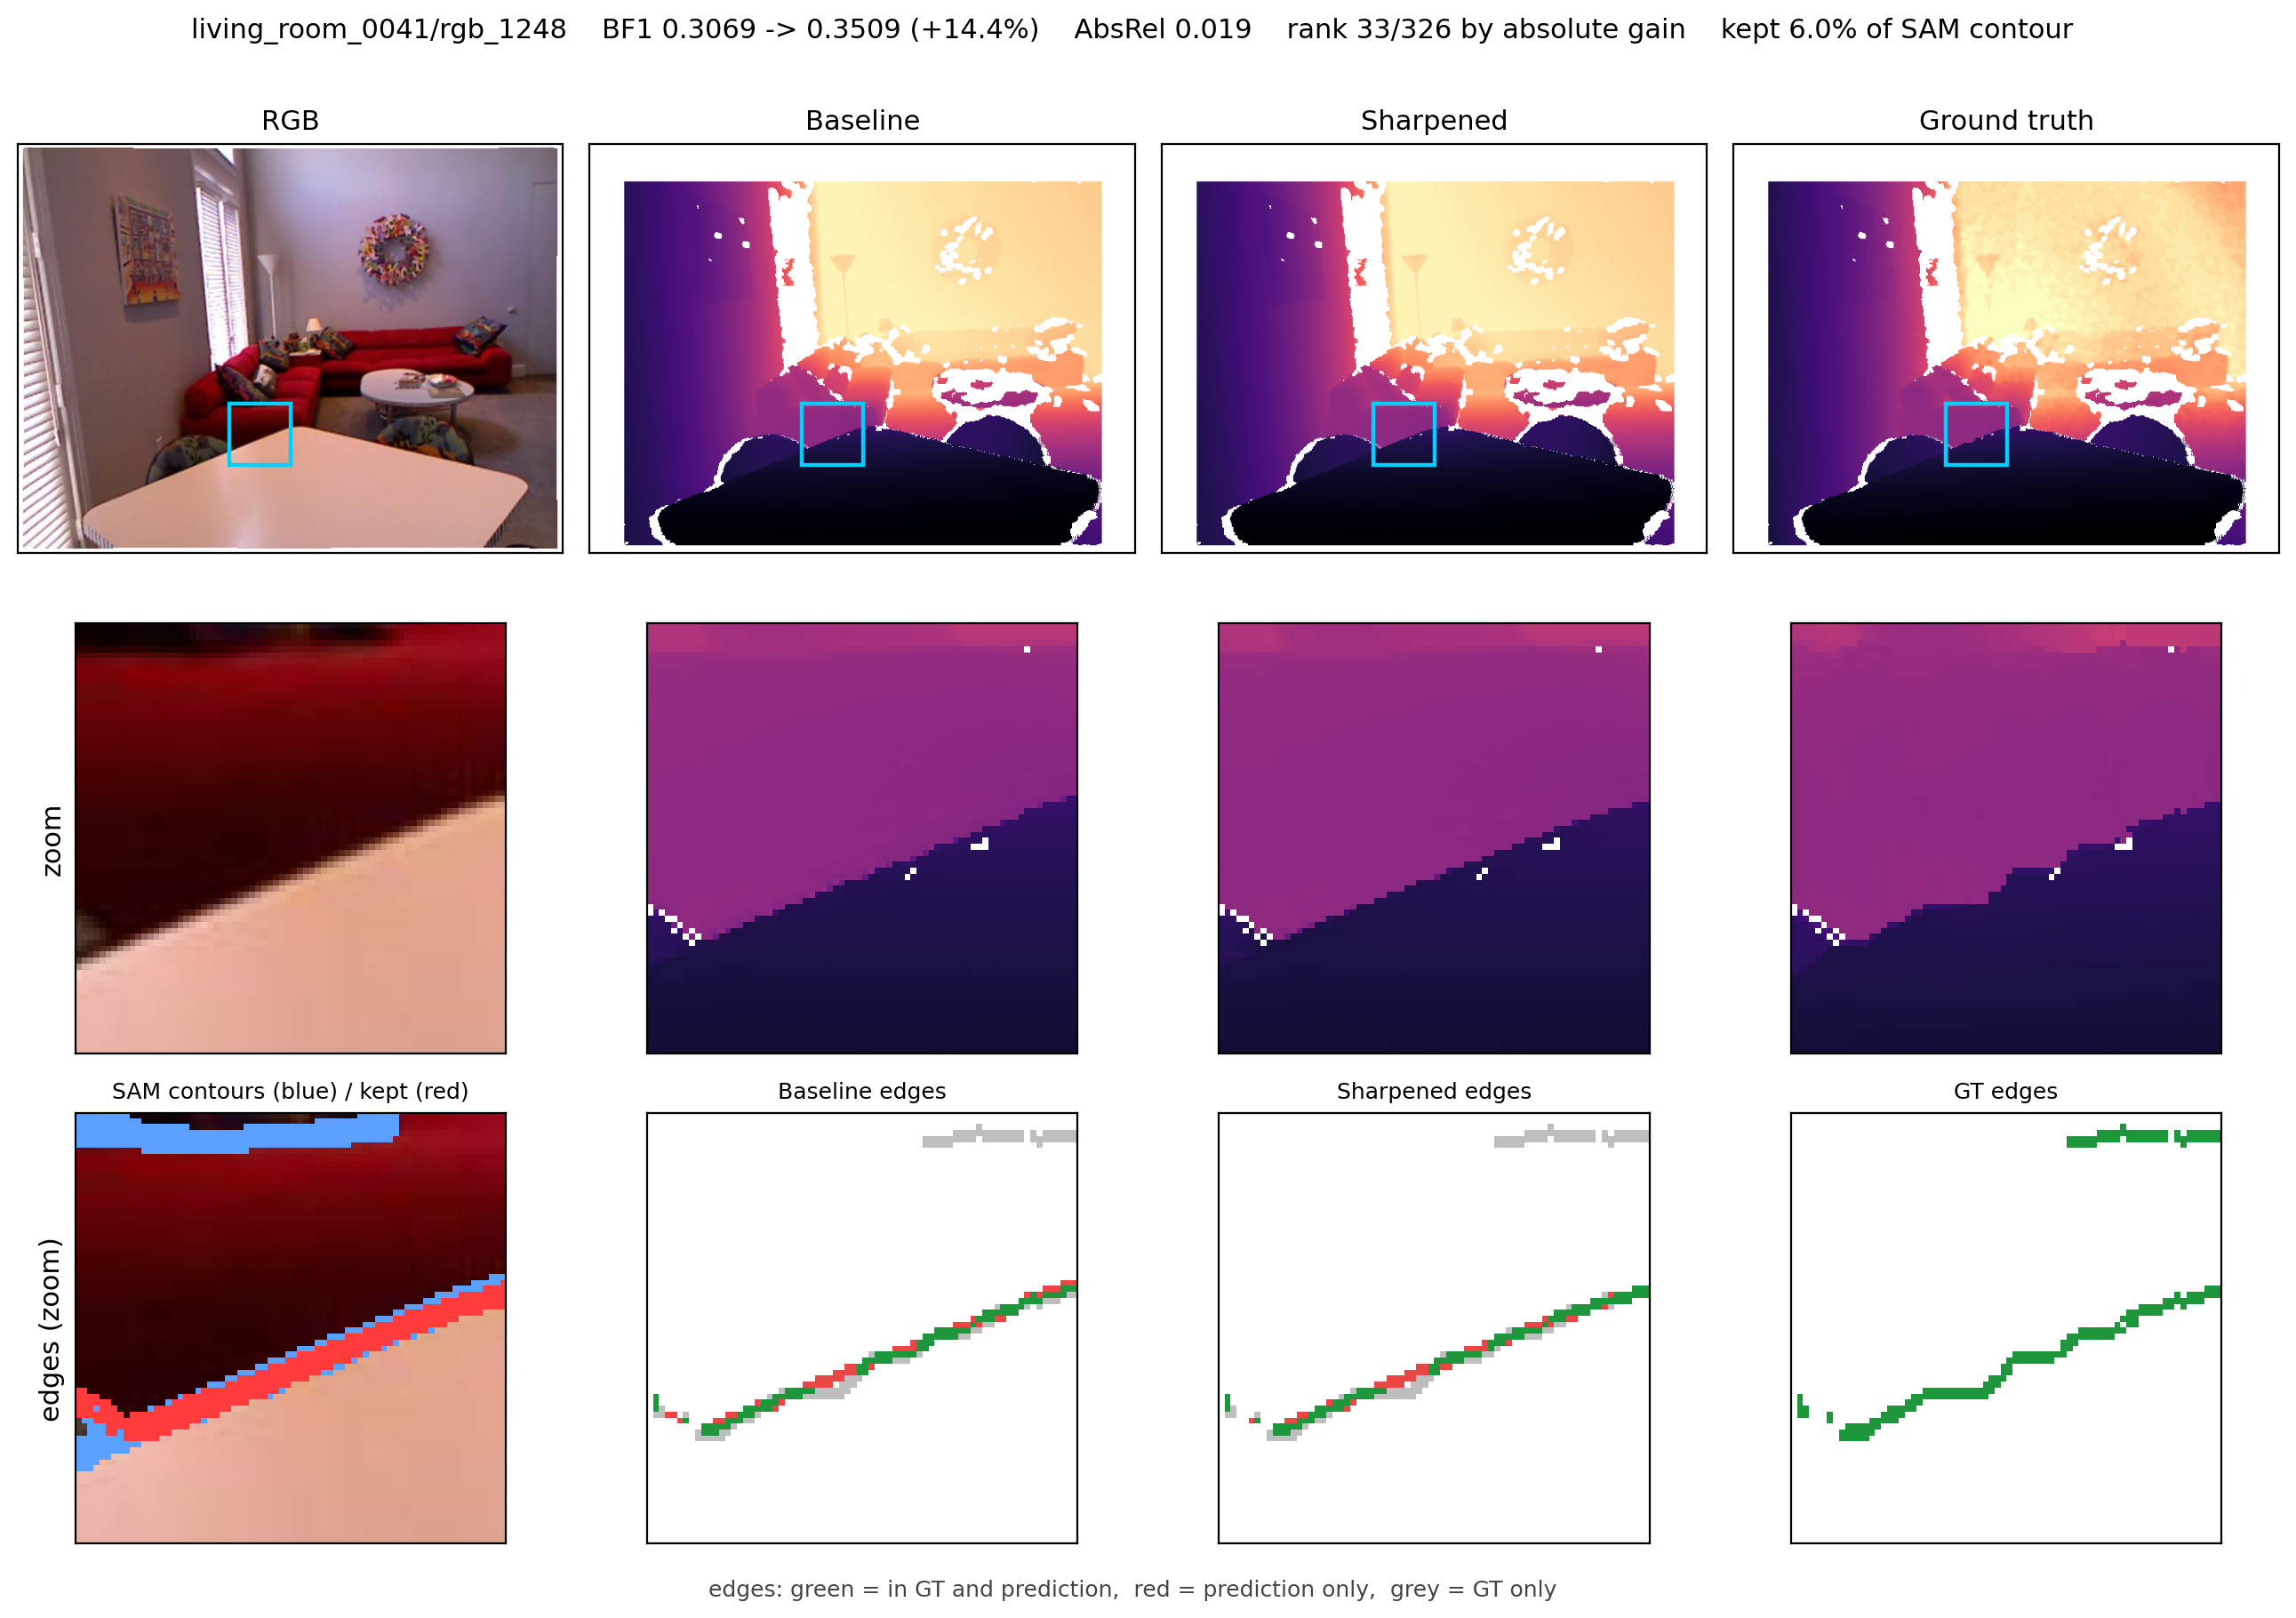
\includegraphics[width=\textwidth]{figures/qualitative_a.png}}
\caption{手法が何をしているか。上段は画像全体で、選別された輪郭の外側は何も
動いていない。中段は 72\,px のズーム。ベースラインでは机の縁が数画素にわたって
にじんでいるのに対し、鋭化後は段差が復元されている。下段は各深度マップが含む
不連続エッジで、これが \bfone{} の比較対象である。緑は正解と予測の両方、
赤は予測のみ、灰は正解のみ。このフレームは、AbsRel が評価集合の中央値 0.0303 以下で
ある 326 枚を\textbf{絶対}利得で並べたときの 33 位である。\textbf{相対}利得で見れば
その $+14.36\%$ は評価集合の中央値 $+13.15\%$ に近い。図を正確な側の半分に限ったのは、
破綻した予測を立て直す例ではなく、良い予測を鋭化する例を示すためである。パネルには各フレームの AbsRel と順位を印字してあり、
分布のどの位置を示しているかを読者が確認できる。}
\label{fig:qualitative}
\end{figure*}

\section{関連研究}

\textbf{拡散ベースの単眼深度推定。}
Marigold \cite{marigold} は Stable Diffusion を合成 RGB-D で微調整し、アフィン不変な
単眼深度推定へ転用した。Marigold V2 \cite{marigoldv2} はその定式化を保ったまま、
U-Net を、画像編集モデルから転用した 213 億パラメータの拡散トランスフォーマに置き換え、
4 bit QLoRA で学習し、1 ステップで推論する。Lotus \cite{lotus} は拡散のスケジュールを取り除き、
タイムステップを固定して 1 ステップで予測する。その後、1 ステップ化が手法を単純化すると
同時に桁違いに高速化することが示された \cite{onestep}。本研究は、この系統の中で可能な限り離れた 2 つのモデルで評価する。
一つは Marigold V2 \cite{marigoldv2}（21{,}282{,}180{,}672 パラメータの
拡散トランスフォーマ、アフィン不変な log 深度を出力）、
もう一つは Lotus \cite{lotus}（8.68 億パラメータの UNet、視差を出力）である。

\textbf{後処理としての境界鋭化。}
Ramamonjisoa らの研究 \cite{ramamonjisoa} が最も近い。遮蔽境界の周囲の画素を再標本化する
2 次元変位場を学習するもので、任意の深度推定器の出力に適用でき、NYUv2 の学習 795 枚・
評価 654 枚という使い方まで本研究と同一である。SharpNet \cite{sharpnet} は遮蔽輪郭の回復を
深度ネットワーク自身の学習に組み込む。Edge-guided 後処理 \cite{edgeguided} は自己教師ありの
視差合成において境界を保存する。より最近では、NeRF による深度精緻化 \cite{nerfrefine} が、単眼推定と再構成された
場を融合して幾何的な細部を回復している。これらはいずれも\emph{深度をどう動かすか}を学習する。
著者らの知る限り、修正操作を固定して対象だけを学習する研究はなく、また
プロンプト可能な分割モデルを境界候補の供給源として用いる研究もない。

\textbf{直接比較は行っていない。} \cite{ramamonjisoa} はコードが公開されているが
学習済み重みの公開がなく、README に推論手順の記載もなく、PyTorch 0.4 系の API に依存しているため、
現行の PyTorch では動作しない。代わりに本研究自身の分割モデルの使い方をアブレーションし
（第 \ref{sec:experiments} 節）、外部の分割モデルがどれだけ寄与するかという関連する問いに答えた。
\textbf{これは本手法のアブレーションであって先行研究との比較ではなく、そのように提示する
こともしない。} 本手法の学習は 16 分で済むため、同じ評価集合で再実装して比較するのが
本来の比較であり、それは今後の課題である。

\textbf{境界指標。}
Depth Pro \cite{depthpro} のスケール不変な境界 \bfone{} を採用する。隣接画素間の深度の
\emph{比}が閾値を超えたときに深度段差があると判定し、その閾値を掃引する指標である。
本研究は新しい指標を提案しない。Lotus も Marigold V2 も NYUv2 の \bfone{} を
報告していないため、ベースラインは著者らが測定した。

\textbf{深度のための領域分割。} Segment Anything \cite{sam} は、深度を事前情報としてマスクを
精緻化する方向で利用されてきた。本研究はこれを逆方向に用いる。学習した選別器が選り分ける
\emph{深度境界の候補}の供給源としてである。

\section{診断：ボトルネックは選別である}
\label{sec:diagnosis}

\subsection{修正操作}
この操作を\emph{障壁鋭化}と呼ぶ。選別された輪郭を、深度を内挿してはならない障壁として
扱うからである。$z$ を予測深度、$C$ を輪郭画素の集合とする。操作は $C$ の周囲
$\pm 2$\,px の帯を捨て、その帯を除いた有効領域の連結成分にラベルを付け
（輪郭の両側が別の成分になる）、ラベルを 1 画素ずつ内側へ伝播させて帯を埋め、
輪郭の両側が帯の内部で接するようにし（一方が他方へ漏れ込まないように）、
捨てた各画素を半径 3\,px 以内にある\emph{自分の成分}の深度の平均で埋め直す。帯を捨てるのは、拡散モデルが境界をまたいで値を内挿するためである。
片側だけから埋め直すことで、この混ざりを除去する。
成分ラベルは輪郭そのものから作るのであって、分割マスクからではない。
この操作は設定値を 2 つ持つだけで、
学習するものは何もない。充填半径は帯より大きくなければならない。さもなければ埋める元が
残らず、操作は何もせずに終わる。

両側が分かれるのは、輪郭が閉じているか画像端に達している場合だけである。画像の内側で
途切れる輪郭では、その先端を回り込んで有効領域がつながるため、そこでは帯の両側が
同一の連結成分に属し、片側からの充填は名目だけになる。選別はこれを増やす方向に働く。
輪郭画素の 6\% を残すと、輪郭は全体の輪ではなく断片になるからである。
いずれも修復を弱める性質であり、本稿のすべての数値にそのまま含まれている。

\subsection{全輪郭に掛けると失敗する}
表 \ref{tab:diagnosis} は、Marigold V2 を土台に、
Segment Anything が描く輪郭すべてにこの操作を掛けた結果である。境界 \bfone{} は
1.90\% 低下する。\textbf{この診断は、境界がすでにある程度正しいモデルに固有である。}
Lotus では同じ無選別の鋭化が逆に 10.31\% \emph{改善}する（表 \ref{tab:controls}）。
ベースライン \bfone{} が 0.0693 と Marigold V2 の 0.0884 より低く、境界がもともと
鈍いぶん、得るものが多く損なうものが少ないからである。選別は前者で操作を安全にし、
両者で大きく改善させる。

\begin{table}[t]
\caption{Marigold V2 で後処理による鋭化が失敗する理由と、何がそれを直すか。
NYUv2 654 枚。オラクル選別は正解データを用いて分割輪郭の部分集合を選ぶもので、
輪郭は 1 画素も動かさない。}
\label{tab:diagnosis}
\centering
\begin{tabular}{lrr}
\toprule
鋭化した輪郭 & 残存率 & \bfone{} の変化 \\
\midrule
分割モデルの全輪郭 & 100\% & $-1.90\%$ \\
オラクル選別（段差から 1\,px 以内） & 6.07\% & $\mathbf{+43.39\%}$ \\
\bottomrule
\end{tabular}
\end{table}

\subsection{位置精度は問題ではない}
真の深度不連続それぞれから最寄りの輪郭までの距離を測ると、中央値 1.00\,px、
66.9\% が 1\,px 以内、76.9\% が 2\,px 以内である。輪郭は境界のある場所にある。
問題は逆方向にあり、\textbf{輪郭画素の 79.8\% は、半径 8 画素の窓の中に深度段差を一つも持たない}
——壁紙の柄、床の目地、ポスターの縁である。
そこを鋭化することは、滑らかな面の帯を捨てて、値の一致する両側から埋め直すことであり、
雑音を加える以外の効果がない。

\subsection{正解で選別すると符号が反転する}
上に出た 2 つの許容距離は同じ量の裏返しではないので、両方を明記する。79.8\% は
各輪郭画素を中心とする半径 8 画素の窓という緩い基準、以下の選別は 1 画素という
厳しい基準である。1 枚あたり
22{,}167 画素ある分割輪郭——有効画素の 10.6\%——のうち、真の不連続から 1\,px 以内に
あるのは 1{,}345 画素、すなわち 6.07\% である。それをちょうど残し、
残した輪郭はすべて元の位置に置いたまま鋭化すると、効果は $-1.90\%$ から
$+43.39\%$ へ動く（表 \ref{tab:diagnosis}）。輪郭は一つも動いていない。変わったのは集合だけである。
これは選別がボトルネックであることを切り分けて示すと同時に、学習する選別器の目標を定める。

\section{手法}
\label{sec:method}

\begin{figure}[t]
\centerline{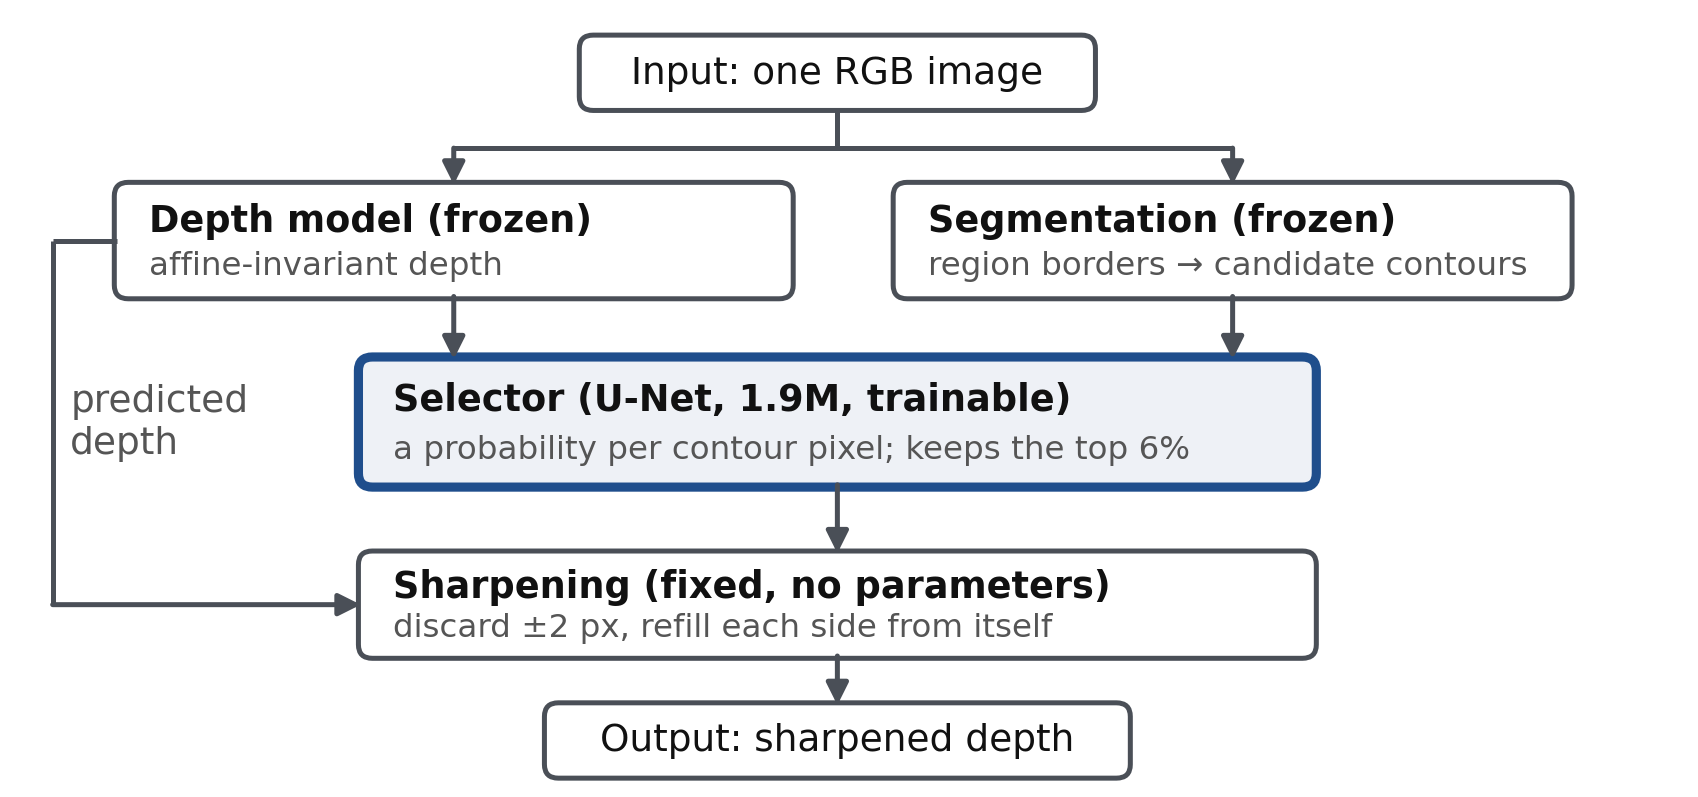
\includegraphics[width=\columnwidth]{figures/pipeline.png}}
\caption{学習するのは選別器だけ。深度推定モデルも分割モデルも凍結し、
修正操作はパラメータを持たない固定操作である。したがって利得は選別のみに帰属する。}
\label{fig:pipeline}
\end{figure}

図 \ref{fig:pipeline} にパイプラインを示す。深度推定モデルと分割モデルは凍結する。
修正は第 \ref{sec:diagnosis} 節の固定操作である。学習する構成要素は選別器だけである。

\textbf{入力と出力。} 選別器は 4 段の U-Net で、パラメータ数は 1{,}928{,}993 である。
RGB 画像（3 チャネル）、予測深度（1）、輪郭マスク（1）を入力し、画素ごとに 1 つの
ロジットを出す。予測深度は\textbf{画像ごとに標準化}する。この手順を省くと、学習時と推論時で水準や尺度が
食い違ってもエラーは生じず、最終的な指標だけが目立たない形で悪化する。
log 深度ではなく視差 $v$ を出すモデルに対しては、先に $-\log\max(v, 10^{-3})$ を適用する。
視差は深度が小さいほど大きくなるためそのまま与えると符号の反転した信号を渡すことになり、
またアフィン不変な視差は 0 以下にもなりうるので、下限でクリップする。
これは深度について単調だが、log 深度のアフィン変換ではない。視差の未知のシフトは
対数を通って非線形性として残り、画像ごとの標準化では落ちない。それでも選別器は
そのまま適用しており、表 \ref{tab:main} の Lotus 列がこの近似の価値である。

\textbf{残存率。} 確率の閾値ではなく、\textbf{画像ごとに上位 6\%} の輪郭画素を残す。
予算を 6\% にしたのは、それが正例率だからである。学習フレームでは輪郭画素の 6.07\% が
真の段差から 1\,px 以内にある。test 集合に合わせたものではない。
閾値を固定すると、場面に含まれる輪郭の量によって残す量が変わり、鋭化が使う予算が
フレームごとに動いてしまう。

\textbf{損失と学習。} 輪郭画素だけにマスクした二値交差エントロピーを用いる。
有効画素のうち輪郭でない 89\% は、選別器に問うていない問題である。輪郭画素は、
正解深度の不連続から 1\,px 以内にあれば正例とする。ここで不連続とは深度比 10\% 超の
段差である。この閾値は test 集合ではなく\textbf{検証集合で選んだ}。学習 795 枚から
外した 40 シーン・141 枚で \bfone{} を測ると、10\% が $+12.74\%$ で、15・20・25\% の
$+8.66$・$+6.29$・$+5.28\%$ を上回る。閾値を上げると正例が輪郭画素の 6.07\% から
2.13\% まで減り、固定の予算がほとんど負例に費やされるためである。
本研究で test 集合を使って選んだものは、第 \ref{sec:controls} 節が明記する対照を除いて
一つもない。それは対照であって手法ではない。\textbf{正解データはこのラベル生成にのみ用い、
推論経路には一切現れない。} NYUv2 の学習用 795 枚をシーン単位で分け、654 枚を学習、
141 枚を検証に充てる。配備するチェックポイントは検証適合率が最良のエポックのもので、
見ているのはこの 654 枚だけであり、評価用の 654 枚とは別の集合である。学習は
RTX 4090 1 枚で 16 分・VRAM 3.5\,GB を要し、評価集合には一度も触れない。

\section{実験}
\label{sec:experiments}

\subsection{設定}
NYUv2 \cite{nyuv2} の評価用 654 枚で評価する。学習フレームとはシーンが重複しない。
第 \ref{sec:limitations} 節の転移先は、\cite{marigoldv2} が用いる ScanNet
\cite{scannet} の検証用 800 枚と、Hypersim \cite{hypersim} のシーン単位ホールドアウト
300 枚である。いずれも深度を 16 bit ミリメートルで保持し、各データセット固有の有効マスクと
深度範囲で読む。NYUv2 のみ Eigen crop を併用する。
指標は Depth Pro \cite{depthpro} のスケール不変な境界 \bfone{} で、5\% から 25\% までの
11 点の閾値で掃引する。各土台モデル自身の未鋭化の予測に対する \bfone{} の相対変化を
相対変化として報告する。予測は採点前にそれぞれの空間——一方は log 深度、他方は視差——で
正解に整合させる。この整合はすべての変種に等しく作用する。

\subsection{主結果}
表 \ref{tab:main} は、アーキテクチャもパラメータ規模も出力表現も共有しない 2 つの
深度モデルでの結果である。seed だけが異なる 4 つの選別器を、すべて Marigold V2 の予測で学習した。
同じ 4 つを Lotus へ\textbf{再学習なしで}適用し、視差から log 深度への変換だけを加えている。
Lotus 側の標準偏差は、\textbf{その 4 つを Lotus に適用したときのばらつき}であって、
Lotus で学習した 4 モデルのばらつきではない。

\begin{table}[t]
\caption{主結果。seed 4 本、$\pm$ は標準偏差。同じ 4 つの選別器を両モデルに適用しており、
学習は第一のモデルでのみ行った。}
\label{tab:main}
\centering
\begin{tabular}{lrrr}
\toprule
土台の深度モデル & \bfone{} & 選別なし & ＋選別器 \\
\midrule
Marigold V2・213 億・log & 0.0884 & $-1.90\%$ & $\mathbf{+11.92 \pm 0.90\%}$ \\
Lotus・8.68 億・視差 & 0.0693 & $+10.31\%$ & $\mathbf{+27.83 \pm 1.27\%}$ \\
\bottomrule
\end{tabular}
\end{table}

第一のモデルでは seed 4 本すべてが $+10\%$ を超え、95\% 信頼区間の下限は $+10.49\%$ である。
画素単位の精度は劣化しない。AbsRel は 0.03881 から 0.03860 へ、$\delta_1$ は 0.97969 から
0.98000 へ動く。いずれも変化は小さく、\textbf{境界のために精度を犠牲にしていない}
ということのみを主張する。

フレーム単位で採点すると、平均が少数のフレームに支えられているのではないことが分かる。
651 枚のうち \textbf{484 枚（74.3\%）で改善}し、相対利得の中央値は $+13.15\%$、
第 1・第 3 四分位は $-0.19\%$ と $+31.57\%$ である。すなわち 4 枚に 1 枚はわずかに
悪化している。ここで除いた 3 枚は、ベースライン \bfone{} が
11 閾値すべてで 0 であり、相対利得が定義できない。プール値には 0 として含まれている。図 \ref{fig:qualitative} はこの分布の中ほどに
あるフレームである。

\subsection{もう一つの境界指標}
一つの指標でしか見えない改善は、その指標の定義による改善かもしれない。そこで
\textbf{Soft Edge Error} でも測った。Marigold V2 \cite{marigoldv2} の著者自身が
使う境界指標で、
その実装から移植した。SEE$_k$ は、正解の境界画素において、$k \times k$ 近傍のどれかの
正解深度との絶対誤差の最小値を平均する。境界のズレは許し、にじみは罰する。
\bfone{} と違って深度単位の絶対誤差なのでスケール不変ではなく、採点前に整合させる必要が
ある。\textbf{小さいほど良い。}

\begin{table}[t]
\caption{Soft Edge Error。表 \ref{tab:main} の 4 seed のうち $+12.49\%$ を出した
1 つ（4 本中 2 番目）を、両モデルにそのまま適用した値。小さいほど良く、\%\ は各モデル自身のベースラインに
対する相対変化。「GT 輪郭」は正解の不連続そのもので鋭化するもので、分割輪郭から選んで
到達できる上限ではない。表 \ref{tab:diagnosis} のオラクル選別はこれとは別の、
はるかに小さい上限である。}
\label{tab:see}
\centering
\begin{tabular}{lrrrr}
\toprule
& \bfone{} & SEE$_3$ & SEE$_5$ & SEE$_7$ \\
\midrule
\multicolumn{5}{l}{\emph{Marigold V2}} \\
ベースライン & 0.0884 & 0.1148 & 0.0882 & 0.0758 \\
＋選別器 & $+12.49\%$ & $-3.34\%$ & $-2.89\%$ & $-2.39\%$ \\
移設対照 & $-0.50\%$ & $+0.32\%$ & $+0.46\%$ & $+0.52\%$ \\
GT 輪郭 & $+209.8\%$ & $-11.44\%$ & $-5.09\%$ & $-2.91\%$ \\
\midrule
\multicolumn{5}{l}{\emph{Lotus}} \\
ベースライン & 0.0693 & 0.1403 & 0.1147 & 0.1014 \\
＋選別器 & $+28.18\%$ & $-5.18\%$ & $-5.54\%$ & $-5.48\%$ \\
移設対照 & $-0.57\%$ & $+0.20\%$ & $+0.23\%$ & $+0.24\%$ \\
GT 輪郭 & $+279.0\%$ & $-12.96\%$ & $-9.81\%$ & $-8.73\%$ \\
\bottomrule
\end{tabular}
\end{table}

\textbf{2 つの指標は、両モデルのすべての変種で一致する。} 選別器は両方で改善、
移設対照は両方で悪化、GT 輪郭での鋭化は両方で最良。したがって\textbf{この改善は \bfone{} の
定義の産物ではない}。

ただし変化の大きさは比較できない。SEE は境界画素の絶対誤差の平均で、その場所での
モデル自身の深度値の精度が下限になる。だから GT 輪郭での鋭化は \bfone{} を $209.8\%$ 上げる一方、
SEE$_5$ は $5.09\%$ しか下げない。また $k$ が大きいほど改善が小さくなる
（GT 輪郭で $-11.44\%$ から $-2.91\%$）。大きい $k$ ほどズレを許すのだから、
そうなるのが定義どおりである。

\subsection{対照}
\label{sec:controls}
利得は学習ではなく鋭化そのものから来ているのかもしれず、あるいは単に疎であることから
来ているのかもしれない。表 \ref{tab:controls} は、学習を伴わない 5 つの代替手段を、
\textbf{各土台モデル自身の予測で}測定したものである。

\begin{table}[t]
\caption{学習を伴わない対照。土台モデルごとに別々に測定した \bfone{} の変化。
移設の行は独立な 3 回の移設の平均、ランダム 2 行は 3 回の抽出の平均で、
いずれも選別器と同じ 1 枚ごとの予算を使う。}
\label{tab:controls}
\centering
\begin{tabular}{lrr}
\toprule
選別の方法 & Marigold V2 & Lotus \\
\midrule
なし（全輪郭） & $-1.90\%$ & $+10.31\%$ \\
移設（同じ疎さ・違う場所） & $-0.50\%$ & $-0.57\%$ \\
画素ランダム & $-24.96 \pm 0.53\%$ & $-22.11 \pm 1.17\%$ \\
ブロックランダム & $-1.04 \pm 0.15\%$ & $-0.03 \pm 0.36\%$ \\
手作り特徴の閾値（最良） & $+1.25\%$ & $+10.46\%$ \\
\midrule
\textbf{学習した選別器} & $\mathbf{+11.92\%}$ & $\mathbf{+27.83\%}$ \\
\textbf{学習の寄与} & $\mathbf{10.7}$\,pt & $\mathbf{17.4}$\,pt \\
\bottomrule
\end{tabular}
\end{table}

手作り特徴の対照は、予測深度の log 勾配の局所的な記述子に閾値を掛けるものである。
その特徴量は、ホールドアウトでの順位付けの良さではなく\textbf{test 集合の最終指標で選んだ}。候補 4 つを測ると
AUC の順位と \bfone{} の順位は\emph{逆転}し、AUC が最も低い特徴量（0.801）が
\bfone{} 最良（$+1.25\%$）を、AUC が最も高い特徴量（0.876）が \bfone{} 最下位
（$-2.59\%$）を与える。これは本手法が持たない優位を対照に与えるので、比較は保守的になる。
代理指標で選んだ対照は弱すぎることになり、
\textbf{弱い対照は比較される手法を良く見せるだけ}である。

ランダム 2 行は、選別器の出力から 1 枚ごとに取った同じ予算をちょうど使う。
画素ランダムが両モデルで近い値（$-24.96\%$ と $-22.11\%$）を示すのは、
この対照が測っているのが鋭化操作の性質であって深度モデルの性質ではないからである。
輪郭を連続させたままのブロックランダムは、どちらでもほとんど損をせず、
Lotus では誤差の範囲で 0 である。画素ランダムをあれほど破壊的にしているのは
\textbf{選択を散らすこと}であり、選び方が悪いこと自体の代償はほとんど無い。

\subsection{分割モデルの寄与}
分割モデルを完全に外し、選別器が RGB と深度から自力で境界を見つけ、有効画素すべてを
候補とする設定では $+7.30\%$ となる。このアブレーションは両方とも単一 seed の値なので、
比較すべきはその seed の $+12.49\%$ である。分割モデルの寄与は 5.19 ポイント、その実行の 42\%
にあたる。その機構は適合率ではなく\textbf{再現率}にある。分割輪郭上で数えると真の段差は
1 枚あたり 1{,}345 画素で、予算 1{,}330 画素はその 98.9\% を覆える。有効画素全体で数えると
2{,}941 画素あり、同じ予算では再現率の上限が 45.2\% になる。
\textbf{分割モデルは正解の集合を絞ることによって寄与している。}

\section{計算コスト}
\label{sec:cost}

表 \ref{tab:cost} は RTX 4090 1 枚での 1 フレームあたりの実時間である。
ウォームアップ後に実フレームで測定した。Marigold V2 のトランスフォーマは、公開設定の
既定である 4 bit NF4 で読み込まれる。したがって 213 億パラメータが占めるのは
およそ 10.6\,GB で、24\,GB のカードに載る。bf16 では載らない。

\begin{table}[t]
\caption{1 枚あたりのコストと、それが買う利得。grid 16 と 48 は表 \ref{tab:main} の
4 seed の平均と標準偏差、他の 2 行はそこで $+12.49\%$ を出した単一 seed の値である。
効いてくる調整項は分割モデルの点グリッドだけである。}
\label{tab:cost}
\centering
\begin{tabular}{lrrr}
\toprule
構成 & ms/枚 & \bfone{} の変化 & 1\,pt あたり \\
\midrule
深度推定モデルのみ & 495 & --- & --- \\
＋選別器（分割なし） & 525 & $+7.30\%$ & \textbf{72} \\
＋選別器・grid 16 & \textbf{1{,}059} & $\mathbf{+11.02 \pm 0.64\%}$ & \textbf{96} \\
＋選別器・grid 32 & 1{,}996 & $+11.17\%$ & 179 \\
＋選別器・grid 48 & 3{,}128 & $+11.92 \pm 0.90\%$ & 262 \\
\bottomrule
\end{tabular}
\end{table}

選別器は 12.0\,ms、鋭化は 18.3\,ms であり、本研究が追加するのは 30.3\,ms——
深度推定モデル自身の 495\,ms の 6\% である。それ以外をすべて支配するのは分割モデルで、
点グリッドに応じて 534\,ms から 2{,}603\,ms を要する。

\textbf{粗いグリッドで十分である。} grid 16 は grid 48 の利得の 92\% を、分割コストの
20\% で達成し、パイプライン全体を 3.0 倍速く、\bfone{} 1 ポイントあたり 2.7 倍安くする。
差の 0.90 ポイントは seed 間の標準偏差 0.90 より小さく、1 組の実行では順序を決められない。
ただし seed で対応をとると grid 48 が 4 本すべてで上回り、差は $0.90 \pm 0.29$ ポイント
（$p = 0.009$）である。差は一貫しており、かつ小さい。
適合率はグリッドをまたいで逆順に並ぶ（grid 16・32・48 で 51.6\%・50.6\%・50.2\%、seed 1 本）。
これは粗いグリッドが何をしているかを示している。大きな物体の輪郭を辿り、壁紙の柄や
床の目地を取りこぼすため、選別器に渡される候補集合の純度がもともと高いのである。
grid 48 は grid 16 より 1 枚あたり 3{,}200 画素多く輪郭を見つけるが、それで買える
\bfone{} は 0.90 ポイントである。増えた輪郭の大半が偽陽性だということである。これは前節のアブレーションと
同じ機構——分割モデルは正解の集合を絞ることで寄与する——が別の軸で現れたものである。

\section{限界}
\label{sec:limitations}

\textbf{公開ベンチマーク 2 つに限ったのは、境界指標が密な正解深度を要求するためである。}
本研究が後処理する土台モデルは、NYUv2・KITTI・ScanNet・ETH3D・DIODE の 5 つで
評価されている。\bfone{} は\emph{隣接画素}の深度比を比較するので、両方が有効である
だけの密度を要し、5 つのうち 3 つはそれを満たさない。KITTI の LiDAR では隣接ペアが
両方有効なのは 13.2\%、ETH3D（レーザー点群を 2440 万画素の DSLR 画像へ投影）では
4.1\% にとどまる。DIODE は密（屋内 99.7\%）だが、レーザー GT が境界で信頼できないため、
標準プロトコルが深度勾配の大きい画素を除外する。そのフィルタは\textbf{深度不連続の
99.4\%（屋内）・100\%（屋外）を取り除く}——本手法が対象とするもの、そのものである。
5 つのうち \bfone{} が定義できるのは NYUv2 と ScanNet であり、本研究はその両方で評価した。
加えて Hypersim でも評価するが、これは 5 つのうちの一つではなく、
Marigold V2 自身の学習ドメインであり、第三の転移テストとして用いる。

\textbf{本手法は深度モデルをまたいでは転移するが、データセットをまたいでは転移しない。}
表 \ref{tab:generalisation} は、NYUv2 で学習した選別器を ScanNet と Hypersim に
適用した結果である（深度モデルは全行で Marigold V2）。

\begin{table}[t]
\caption{汎化。選別器は NYUv2 で学習しており、深度モデルは全行で Marigold V2 である。
適合率はいずれも同じ残存率 6\% で測った。}
\label{tab:generalisation}
\centering
\begin{tabular}{lrrr}
\toprule
評価データ & 選別なし & ＋選別器 & 適合率 \\
\midrule
NYUv2（在ドメイン） & $-1.90\%$ & $\mathbf{+11.92\%}$ & 50.2\% \\
ScanNet & $+3.26\%$ & $+2.81\%$ & 17.4\% \\
Hypersim & $+2.28\%$ & $-4.64\%$ & 55.8\% \\
\bottomrule
\end{tabular}
\end{table}

いずれの未見データセットでも、選別器は全輪郭を使う場合に及ばない。失敗しているのは
\textbf{転移}であって、データセットの側ではない。Hypersim 10{,}000 枚で学習した選別器は、
Hypersim 自身では $+5.05\%$ に達する（選別なしは $+2.28\%$、適合率 88.1\%、
正例率 22.8\%）。同じチェックポイントは NYUv2 で $-2.23\%$、ScanNet で $+0.39\%$ である。
Hypersim も飽和していない——自身の GT 輪郭で鋭化すると $+39.49\%$ になる——ので、
本手法は NYUv2 と同様に Hypersim の在ドメインでも働き、学習と利用でドメインが
変わったときにだけ働かなくなる。

残る 3 通りの対処は失敗した。RGB チャネルを落とすと、転移はむしろ悪化した。
ScanNet で残存率を 2\% から 20\% まで掃引しても、選別なしに届く設定は無かった。
NYUv2 795 枚と Hypersim 795 枚を等量混合して学習すると、在ドメインの結果を損ない、
転移も改善しなかった。\textbf{データ量では転移の失敗を説明できない。} ただし無料でも
ない。NYUv2 を 393 枚に削ると適合率は 3.2 ポイント（50.2\% から 47.0\%）、利得は
2.2 ポイント（$+11.92\%$ から $+9.72\%$、全体の 18\%）下がる。これは seed 2 本での
測定で、表 \ref{tab:main} の 4 本とは本数が違う。一方、在ドメインと ScanNet の差は
9.1 ポイントあり、4 倍大きい。

これを報告するのは、この分野の先行研究が行う主張に関わるからである。
\textbf{モデル非依存な後処理が、それゆえにデータセット非依存であるとは限らない。}
2 種類の汎化は明らかに分離する。

\textbf{適合率は 3 行を並べない。} NYUv2 で学習した選別器は、在ドメインよりも
Hypersim で適合率が高い（50.2\% に対し 55.8\%）のに、結果はそこで最悪である。
そもそも適合率はデータセットをまたいで比較できない。輪郭画素のうち真の段差に
乗っている割合が異なり、NYUv2 の 6.07\% に対し Hypersim は 22.8\% である。
3 行を分けているのは、評価データが選別器の学習ドメインと一致するかどうかであり、
それを測れる量に還元することは著者らにはできていない。

\textbf{上限までの余地。} 第 \ref{sec:diagnosis} 節のオラクル選別は $+43.39\%$ に
達するのに対し、本手法は $+11.92\%$ であり、選別が与えうるものの 72.5\% が未回収である。
差は適合率にある（50.2\% 対オラクルの 100\%）。

\textbf{指標の範囲。} 改善しているのは境界指標である。AbsRel と $\delta_1$ の変化は
改善と主張するには小さすぎ、劣化していないことのみを主張する。

\textbf{ラベルと指標が定義を共有している。} 教師は「正解の深度段差から 1\,px 以内」であり、
\bfone{} も正解の深度段差との一致を測る。正解データは推論に一切現れず、評価シーンは
学習と重複しないが、この対応関係は念頭に置いて読まれるべきである。

\section{おわりに}

単眼深度に対する後処理の境界鋭化が、境界のすでに整ったモデルで失敗するのは、
輪郭の位置が悪いからではなく、その大半が深度段差を示していないからである。修正操作を固定して対象だけを学習することで、
利得の帰属が明確になり、1 枚あたり 30\,ms・193 万パラメータで、再学習なしに深度モデルを
またいで転移する。依存する領域分割は、最も粗いグリッドでもさらに 534\,ms を要する。データセットをまたいでは転移せず、著者らはそれを修復できなかった。

\begin{thebibliography}{00}

\bibitem{marigold} B.~Ke, A.~Obukhov, S.~Huang, N.~Metzger, R.~C.~Daudt, and
K.~Schindler, ``Repurposing diffusion-based image generators for monocular depth
estimation,'' in \emph{CVPR}, 2024.

\bibitem{lotus} J.~He, H.~Li, W.~Yin et al., ``Lotus: Diffusion-based visual
foundation model for high-quality dense prediction,'' in \emph{ICLR}, 2025.

\bibitem{marigoldv2} I.~Pavlovic, T.~Wandel, A.~Obukhov, L.~Bartolomei,
A.~Davydov, F.~Tosi, M.~Poggi, S.~S\"usstrunk, and D.~Dai, ``Marigold V2:
Revisiting diffusion transformers for monocular depth estimation,''
arXiv:2609.08084, 2026.

\bibitem{onestep} G.~M.~Garcia, K.~Knaebel, C.~Schmidt, D.~de~Geus,
A.~Hermans, and B.~Leibe, ``Fine-tuning image-conditional diffusion models is
easier than you think,'' in \emph{WACV}, 2025.

\bibitem{depthpro} A.~Bochkovskii et al., ``Depth Pro: Sharp monocular metric
depth in less than a second,'' in \emph{ICLR}, 2025.

\bibitem{ramamonjisoa} M.~Ramamonjisoa, Y.~Du, and V.~Lepetit, ``Predicting
sharp and accurate occlusion boundaries in monocular depth estimation using
displacement fields,'' in \emph{CVPR}, 2020.

\bibitem{sharpnet} M.~Ramamonjisoa and V.~Lepetit, ``SharpNet: Fast and accurate
recovery of occluding contours in monocular depth estimation,'' in \emph{ICCV
Workshops}, 2019.

\bibitem{edgeguided} K.-S.~Peng, G.~Ditzler, and J.~Rozenblit, ``Edge-guided
occlusion fading reduction for a light-weighted self-supervised monocular depth
estimation,'' arXiv:1911.11705, 2019.

\bibitem{nerfrefine} A.~Muthukkumar, ``Bayesian monocular depth refinement via
neural radiance fields,'' in \emph{Proc. IEEE 8th Int. Conf. Algorithms,
Computing and Artificial Intelligence (ACAI)}, 2025, pp.~488--492.

\bibitem{sam} A.~Kirillov et al., ``Segment Anything,'' in \emph{ICCV}, 2023.

\bibitem{nyuv2} N.~Silberman, D.~Hoiem, P.~Kohli, and R.~Fergus, ``Indoor
segmentation and support inference from RGBD images,'' in \emph{ECCV}, 2012.

\bibitem{scannet} A.~Dai, A.~X.~Chang, M.~Savva, M.~Halber, T.~Funkhouser, and
M.~Nie{\ss}ner, ``ScanNet: Richly-annotated 3D reconstructions of indoor
scenes,'' in \emph{CVPR}, 2017.

\bibitem{hypersim} M.~Roberts et al., ``Hypersim: A photorealistic synthetic
dataset for holistic indoor scene understanding,'' in \emph{ICCV}, 2021.

\end{thebibliography}

\end{document}
